\chapter{Introduction}
\label{ch:introduction}

The involvement of computers in the creation, performance, distribution, and analysis of music is most certainly something that most everyone is aware of regardless of their experience in using these technologies.  Since the creation of the computer, musicians, researchers, and creative people alike have found new and innovative ways to integrate technology into the field of music.

\vspace{\baselineskip}

Some of these innovations that were state of the art at the time that now seem common place include digital audio recording, synthesizers, and music notation software.  As we further advance computers and digital music, we will create and discover new methods to integrate technology into music and find ways to improve our existing means of integration.

\vspace{\baselineskip}

Currently, in the field of computer science, artificial intelligence is being heavily developed and researched.  Its uses, implications, practicality, and future are an important topic of discussion in our lives today.  Specifically related to the uses of AI, artists and musicians are examining ways in which it can be applied to their own processes.

\vspace{\baselineskip}

When the idea of computers creating art and music with computers was initially conceived, the field of AI was nonexistent.  Today, the development of AI has improved extensively, but does not come without limitations.  However, it is now possible to train computers to create and develop original works of both music and art.

\vspace{\baselineskip}

A parallel idea would then be to use computers to teach humans music.  This project set out to try to accomplish this task by creating a computer system that is capable of assisting a person in the creation and validation of a melody.  It was designed in such a way to allow a person with any degree of music or computer knowledge to be able to compose a melody and receive feedback and instruction for how to improve it.

\section{Background}
\label{sec:background}

The earliest cited example of a musical composition that was created using a computer was Hiller and Isaacson's \textit{Illiac Suite} \cite{Fernandez_2013}.  This work was composed in 1956 by Lejaren Hiller and Leonard Isaacson \cite{Brit_2018}.  The following diagram shows the rules that were programmed into the system to guide the composition \cite{Hiller_1992}.  The system of rules that they developed were meant to adhere to the format of strict counterpoint from the Baroque period \cite{Hiller_1992}.  These rules cover cadences, resolutions, voice leading, and voice spacing.

\begin{figure}[!htbp]
	\centering
	\caption{Diagram from Hiller and Isaacson's published paper on the Illiac Suite showing counterpoint rules \cite{Hiller_1992}}
	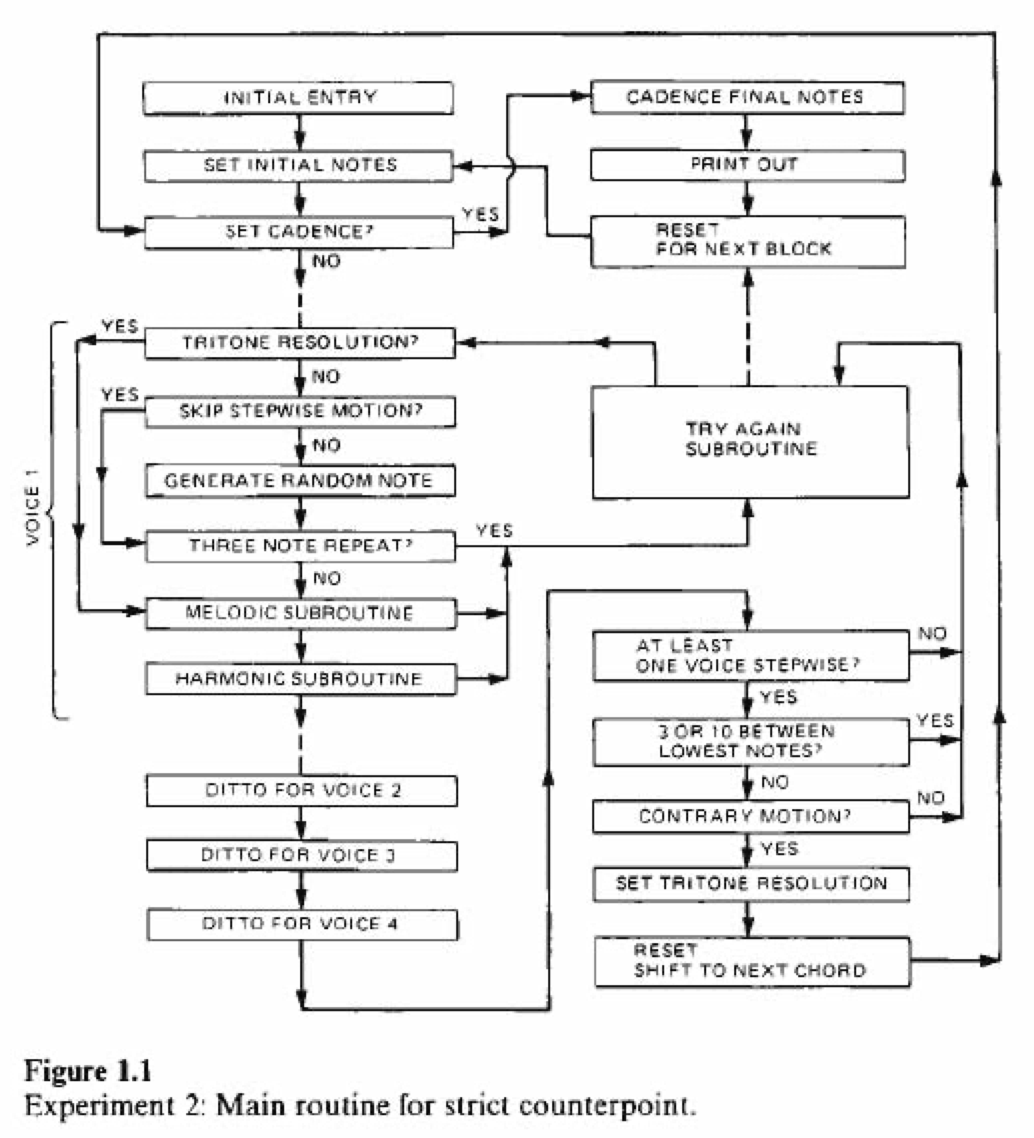
\includegraphics[width=\textwidth]{images/illiacChart}
\end{figure}

\pagebreak

An example of a later approach to computer music composition was Hiller and John Cage's HPSCHD in 1968 \cite{Brit_2018}.  This work was composed by using computers that played Mozart's Musical Dice Game and altered the results using the rules of the Chinese oracle, I Ching \cite{Brit_2018}.

\vspace{\baselineskip}

The development of each of these works required extensive music composition and computer programming knowledge to complete.  Lejaren Hiller was a composer by trade and Leonard Isaacson was a professor of computer science \cite{Brit_2018}.  Neither of these qualifications are applicable to describe the general population of people that are interested in music.  Music has an infinitely deep reaching appeal to practically all humans and even many animals.

\vspace{\baselineskip}

With that being said, it only makes sense then that people who are not educated in either music or computer science should be provided with a way to create music.  By not providing the means for these people to express themselves musically, we miss out on a large amount of creative output and new musical compositions.  Rather than requiring these people to try to gain access to training, we can assist them in musical composition with computer based technology.

\section{Motivation} 
\label{sec:motivation}

Imagine that the piano was an instrument that could only be played if you were over seven feet tall.  If the instrument were designed like this, only a very small portion of the population would be able to make use of it.  The piano, however, is one of the most universally played instruments because it was not designed in a way that excludes lots of people from using it.

\vspace{\baselineskip}

Currently, the tools that exist for computer assisted music composition are only accessible to musicians with high level computer science training \cite{Teymuri_2019}.  All of them either have generally inaccessible command line interfaces or require the user to be trained in music composition to be able to understand or use the output of the program.  Neither of these situation cater to the general person who might find some interest in being able to express themselves by composing with these tools.

\vspace{\baselineskip}

Due to the research heavy focus around the creation of these tools, not a single one was designed to be placed in the hands of the average user.  Someone who may have always wanted to create music might not have access to the training, schooling, tools, or opportunities that are currently required to be able to compose, record, or play music.  Giving these people a tool that can help them through the composition process and assist them in notating their music is an important first step in being able to make creating music more accessible to the average person.

\section{Goals of the Project}
\label{sec:goalsoftheproject}

The goal of this project was to create a computer based musical composition tool that can be used by any person and does not require music or computer science knowledge.  Through the careful design and testing of a user interface built over the high level functions of the composer, this project set out to create a tool that makes music composition accessible to everyone.

\vspace{\baselineskip}

In order to make this a reality, the project was broken into three main components.

\begin{enumerate}
	\item Computer Composer Development
	\item User Interface Development
	\item User Experience Study
\end{enumerate}

\subsection{Computer Composer Development}
\label{subsec:computercomposerdevelopment}

This part of the project consisted of developing the backend functions of the computer composer.  Several different preexisting tools were combined to create the composer and to process its output.  The basic primary functions of the composer include melody generation, notation, playback, analysis, and output.

\vspace{\baselineskip}

Each of these is a necessary part of the tool in order to make the composer into one that covers all of the bases of musical composition.  After the generation of the musical output, the user is free to do what they would like in changing and altering it either with the composer or externally.

\subsection{User Interface Development}
\label{subsec:userinterfacedevelopment}

This next part of the project consisted of building the interface that the user would use to interact with the composer.  There are already several tools that perform some combination of the functions of the composer that were listed above, but none of them have this interface component.

\vspace{\baselineskip}

In order to meet the overall goal and motivation for this project, the interface had to be designed in a way that could, in essence, explain itself.  Rather than having long lists of instructions and using lost of music theory terminology, the interface has to present itself in a way that each element explains its own function in a completely visual way.  This is where the bulk of the work of the project was done.

\subsection{User Experience Study}
\label{subsec:userexperiencestudy}

Following the development of the composer and the UI, it was necessary to test the effectiveness of the UI and if it met the idea behind the project through a user study.   Users with varying degrees of musical knowledge were asked about their experiences through interacting with the tool.  The overall success of the interface design was gauged through a series of survey questions.

\vspace{\baselineskip}

After getting feedback from users of the tool, some revisions were performed to the interface to clear up uncertainties and confusions that the users had.  This is an important step in UI development since not every user of the interface is going to see it or interact with it in the same way.

\section{Thesis Outline}
\label{sec:thesisoutline}

The following outlines what is contained within this thesis document.

\subsection{Introduction}
\label{subsec:thesisoutlineintroduction}

This section of the document provides the situating of the work within the disciplines of music and computer science.  It contains details about the history of computer composed music and some background into the associated problems.  It also discusses the motivation for the project and its overall goals.

\subsection{Related Work}
\label{subsec:thesisoutlinerelatedwork}

This section of the thesis document provides a discussion into the other published works related to computer composed music.  It discusses the details and ideas used in these projects as well as some of their shortcomings as related to the motivation behind this project.

\subsection{Method of Approach}
\label{subsec:thesisoutlinemethodofapproach}

This section details the approach taken to solve the problem discussed during the introduction.  It explains the composer and user interface development.  It further discusses the reasons for these parts of the project and what was entailed in their completion.

\subsection{Experimental Results}
\label{subsec:thesisoutlineexperimentalresults}

This section of the document provides a discussion of the user study and the overall successes and failures of the project.  It summarizes the users' responses to the questions in the study and what their responses mean for the evaluation of the system.

\subsection{Discussion and Future Work}
\label{subsec:thesisoutlinediscusionandfuturework}

This section of the thesis document discusses the overall impact of this project and what might be done in the future to improve it.  Neither of these are limited to strictly the research based impact of this project as the goal of this project is to move the tool beyond the lab and into the hands of the average user.